%%%%%%%%%%%%%%%%%%%%%%%%%%%%%%%%%%%%%%%%%
% Programming/Coding Assignment
% LaTeX Template
%
% This template has been downloaded from:
% http://www.latextemplates.com
%
% Original author:
% Ted Pavlic (http://www.tedpavlic.com)
%
% Note:
% The \lipsum[#] commands throughout this template generate dummy text
% to fill the template out. These commands should all be removed when 
% writing assignment content.
%
% This template uses a Perl script as an example snippet of code, most other
% languages are also usable. Configure them in the "CODE INCLUSION 
% CONFIGURATION" section.
%
%%%%%%%%%%%%%%%%%%%%%%%%%%%%%%%%%%%%%%%%%

%----------------------------------------------------------------------------------------
%	PACKAGES AND OTHER DOCUMENT CONFIGURATIONS
%----------------------------------------------------------------------------------------

\documentclass[11pt,norsk,a4paper]{article}

\usepackage{ucs,babel}
\usepackage{fancyhdr} % Required for custom headers
\usepackage{lastpage} % Required to determine the last page for the footer
\usepackage{extramarks} % Required for headers and footers
\usepackage[usenames,dvipsnames]{color} % Required for custom colors
\usepackage{graphicx} % Required to insert images
\usepackage{listings} % Required for insertion of code
\usepackage{courier} % Required for the courier font
\usepackage{lipsum} % Used for inserting dummy 'Lorem ipsum' text into the template
\usepackage[utf8]{inputenc} %For "spesielle" tegn som æ, ø, å og andre er det anbefalt å angi dette. Mac brukere kan vurdere applemac og ikke utf8
\usepackage{amssymb}



% Margins
\topmargin=-0.45in
\evensidemargin=0.75in
\oddsidemargin=0.75in
\textwidth=5in
\textheight=9.0in
\headsep=0.25in

\linespread{1.1} % Line spacing

% Set up the header and footer
\pagestyle{fancy}
\lhead{\hmwkAuthorName} % Top left header
\rhead{ \hmwkTitle} % Top center head
%\rhead{\firstxmark} % Top right header
\lfoot{\lastxmark} % Bottom left footer
\cfoot{} % Bottom center footer
\rfoot{Side\ \thepage\ av\ \protect\pageref{LastPage}} % Bottom right footer
\renewcommand\headrulewidth{0.4pt} % Size of the header rule
\renewcommand\footrulewidth{0.4pt} % Size of the footer rule

%\setlength\parindent{0pt} % Removes all indentation from paragraphs

\usepackage{empheq}
\usepackage[dvipsnames,table]{xcolor}
\definecolor{medGray}{RGB}{230,230,230}

\newenvironment{important}[2][]{
\setkeys{EmphEqEnv}{#2}
\setkeys{EmphEqOpt}{box={\setlength{\fboxsep}{10pt}\colorbox{medGray}},#1}
\EmphEqMainEnv}
{\endEmphEqMainEnv}

%----------------------------------------------------------------------------------------
%	CODE INCLUSION CONFIGURATION
%----------------------------------------------------------------------------------------

\definecolor{MyDarkGreen}{rgb}{0.0,0.4,0.0} % This is the color used for comments
\lstloadlanguages{Perl} % Load Perl syntax for listings, for a list of other languages supported see: ftp://ftp.tex.ac.uk/tex-archive/macros/latex/contrib/listings/listings.pdf
\lstset{language=Perl, % Use Perl in this example
        frame=single, % Single frame around code
        basicstyle=\small\ttfamily, % Use small true type font
        keywordstyle=[1]\color{Blue}\bf, % Perl functions bold and blue
        keywordstyle=[2]\color{Purple}, % Perl function arguments purple
        keywordstyle=[3]\color{Blue}\underbar, % Custom functions underlined and blue
        identifierstyle=, % Nothing special about identifiers                                         
        commentstyle=\usefont{T1}{pcr}{m}{sl}\color{MyDarkGreen}\small, % Comments small dark green courier font
        stringstyle=\color{Purple}, % Strings are purple
        showstringspaces=false, % Don't put marks in string spaces
        tabsize=5, % 5 spaces per tab
        %
        % Put standard Perl functions not included in the default language here
        morekeywords={rand},
        %
        % Put Perl function parameters here
        morekeywords=[2]{on, off, interp},
        %
        % Put user defined functions here
        morekeywords=[3]{test},
       	%
        morecomment=[l][\color{Blue}]{...}, % Line continuation (...) like blue comment
        numbers=left, % Line numbers on left
        firstnumber=1, % Line numbers start with line 1
        numberstyle=\tiny\color{Blue}, % Line numbers are blue and small
        stepnumber=5 % Line numbers go in steps of 5
        }

% Creates a new command to include a perl script, the first parameter is the filename of the script (without .pl), the second parameter is the caption
\newcommand{\perlscript}[2]{
\begin{itemize}
\item[]\lstinputlisting[caption=#2,label=#1]{#1.pl}
\end{itemize}
}

%----------------------------------------------------------------------------------------
%	DOCUMENT STRUCTURE COMMANDS
%	Skip this unless you know what you're doing
%----------------------------------------------------------------------------------------

% Header and footer for when a page split occurs within a problem environment
\newcommand{\enterProblemHeader}[1]{
\nobreak\extramarks{#1}{#1 continued on next page\ldots}\nobreak
\nobreak\extramarks{#1 (continued)}{#1 continued on next page\ldots}\nobreak
}

% Header and footer for when a page split occurs between problem environments
\newcommand{\exitProblemHeader}[1]{
\nobreak\extramarks{#1 (continued)}{#1 continued on next page\ldots}\nobreak
\nobreak\extramarks{#1}{}\nobreak
}

\setcounter{secnumdepth}{0} % Removes default section numbers
\newcounter{homeworkProblemCounter} % Creates a counter to keep track of the number of problems

\newcommand{\homeworkProblemName}{}
\newenvironment{homeworkProblem}[1][Problem \arabic{homeworkProblemCounter}]{ % Makes a new environment called homeworkProblem which takes 1 argument (custom name) but the default is "Problem #"
\stepcounter{homeworkProblemCounter} % Increase counter for number of problems
\renewcommand{\homeworkProblemName}{#1} % Assign \homeworkProblemName the name of the problem
\section{\homeworkProblemName} % Make a section in the document with the custom problem count
\enterProblemHeader{\homeworkProblemName} % Header and footer within the environment
}{
\exitProblemHeader{\homeworkProblemName} % Header and footer after the environment
}

\newcommand{\problemAnswer}[1]{ % Defines the problem answer command with the content as the only argument
\noindent\framebox[\columnwidth][c]{\begin{minipage}{0.98\columnwidth}#1\end{minipage}} % Makes the box around the problem answer and puts the content inside
}

\newcommand{\homeworkSectionName}{}
\newenvironment{homeworkSection}[1]{ % New environment for sections within homework problems, takes 1 argument - the name of the section
\renewcommand{\homeworkSectionName}{#1} % Assign \homeworkSectionName to the name of the section from the environment argument
\subsection{\homeworkSectionName} % Make a subsection with the custom name of the subsection
\enterProblemHeader{\homeworkProblemName\ [\homeworkSectionName]} % Header and footer within the environment
}{
\enterProblemHeader{\homeworkProblemName} % Header and footer after the environment
}

%----------------------------------------------------------------------------------------
%	NAME AND CLASS SECTION
%----------------------------------------------------------------------------------------

\newcommand{\hmwkTitle}{Øving\ \#6} % Assignment title
\newcommand{\hmwkDueDate}{Mandag,\ 15\ April,\ 2013} % Due date
\newcommand{\hmwkClass}{TMA4280\ } % Course/class
\newcommand{\hmwkClassTime}{} % Class/lecture time
\newcommand{\hmwkClassInstructor}{} % Teacher/lecturer
\newcommand{\hmwkAuthorName}{Simen Haugerud Granlund \&\ Steffen Pøhner Henriksen} % Your name

%----------------------------------------------------------------------------------------
%	TITLE PAGE
%----------------------------------------------------------------------------------------

\title{
\vspace{2in}
\textmd{\textbf{\hmwkClass:\ \hmwkTitle}}\\
\normalsize\vspace{0.1in}\small{Innleveringsdato\ \hmwkDueDate}\\
\vspace{0.1in}\large{\textit{\hmwkClassInstructor\ \hmwkClassTime}}
\vspace{3in}
}

\author{\textbf{\hmwkAuthorName}}
\date{} % Insert date here if you want it to appear below your name

%----------------------------------------------------------------------------------------

\begin{document}

\maketitle

%----------------------------------------------------------------------------------------
%	TABLE OF CONTENTS
%----------------------------------------------------------------------------------------

%\setcounter{tocdepth}{1} % Uncomment this line if you don't want subsections listed in the ToC

% \newpage
% \tableofcontents
\newpage

%----------------------------------------------------------------------------------------
%	SOLUTION
%----------------------------------------------------------------------------------------

% To have just one problem per page, simply put a \clearpage after each problem
\section{Diskretisering av Poissons ligning}

Programmet skal kunne løse Poisson-ligningen i domenet $ x= [0..1], y = [0..1]. $ Poisson-ligningen er på formen:

\begin{equation} 
-\Delta^2\phi = f(x,y)
\end{equation}
\begin{equation}
-\Delta^2\phi = -\frac{\partial^2\phi}{\partial x^2} - \frac{\partial^2\phi}{\partial x^2} = -u_{xx}-u_{yy} = f(x,y)
\end{equation}

Vi trenger en form av denne som kan løses numerisk. Den må diskretiseres slik at en datamaskin skal kunne løse den. For å få til dette forsøker vi å Taylor-utvikle i  x-, og y-retning. Viser kun utviklingen i x-retning da utregningene er tilsvarende for y.

\begin{equation}
u(x+h,y) = u(x,y) + hu_x(x,y) + \frac{1}{2}h^2u_{xx}(x,y) + \frac{1}{6}h^3u_{xxx}(x,y)+ ...
\end{equation}
\begin{equation}
u(x-h,y) = u(x,y) - hu_x(x,y) + \frac{1}{2}h^2u_{xx}(x,y)- \frac{1}{6}h^3u_{xxx}(x,y)+ ...
\end{equation}

Vi ser bortifra høyere ordens ledd ($h^3, h^4$...), og løser for $u_{xx}$.

\begin{equation}
u_{xx}(x,y) \approx \frac{1}{h^2}(u(x+h,y)-2u(x,y)+u(x-h,y))
\end{equation}

Dermed har vi nå et uttrykk for $u_{xx}$ som er lettere å forstå for en datamaskin. Tilsvarende har vi et uttrykk for $u_{yy}$. Vi legger disse sammen og får et diskretisert uttrykk for Poisson-ligningen, også kalt fem-punktsformelen.

\begin{important}{equation}
-u(x+h,y)-u(x,y+h)-u(x-h,y)-u(x,y-h)+4u(x,y) = h^2f(x,y)
\end{important}

I (6) betegner $f$ hvor finkjemmet rutenett som benyttes (steglengden). Det diskretiserte uttrykket løser problemet i punkt for punkt, og tettheten til punktskyen avhenger av h. Vi kan se at hvert punkt avhenger av nabopunktene (firer-naboer) i x- og y-retning både negativt og positivt. Utifra den observasjonen kan vi sette opp et stensil som gjør det enklere å se hva den betyr.

\begin{figure}[h]
\centering
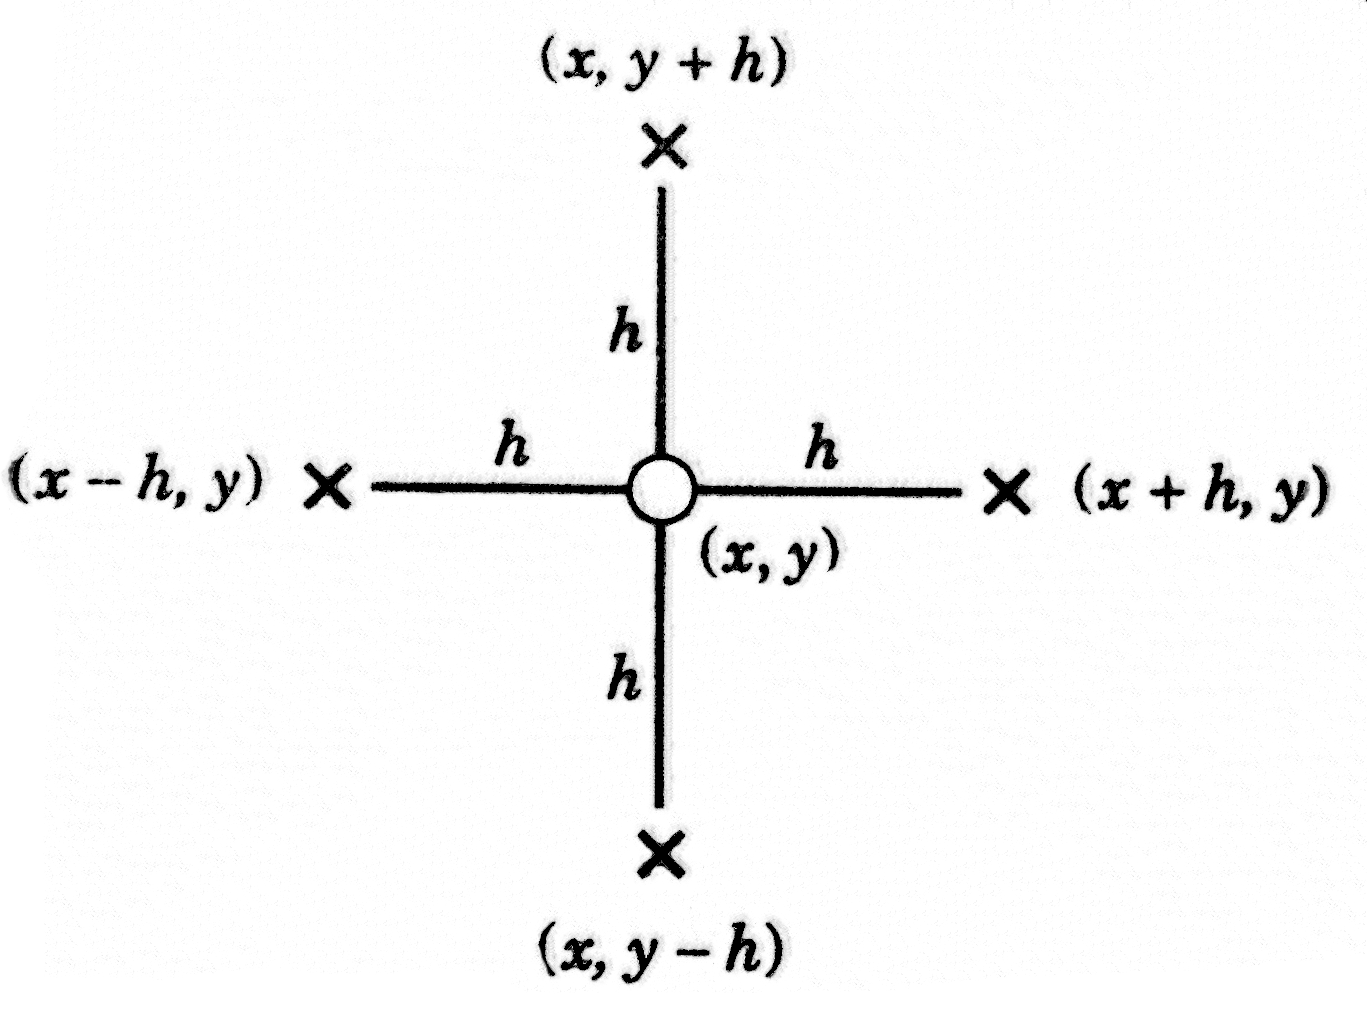
\includegraphics[scale=0.2]{five.png}
\caption{Fem-punkts stensil \cite{ky}}
\end{figure}

Utifra stensilen kan vi sette opp en ligning for hvert punkt. Høyresiden blir $h^2f(x,y)$ hvor x og y betegner posisjonen til punktet vi ser på i domenet. Venstresiden refererer til hvert nabopunkt en gang, og til seg selv 4 ganger. Om et refererende punkt ligger på grensen til domenet ersattes dette med grensebetingelsen, f.eks 0 ved Dirichlet-betingelser.

Vi kan sette ligningene sammen til et system på formen \textbf{Ax = b}. Som kan løses av en datamaskin på mange måter. Antall punkt, og dermed antall ligninger, avhenger av $h$, og vokser i graden $h^2$. Det betyr at dersom vi dobler antall punkt, firedobler vi antall ligninger maskinen må løse. 

\section{Løsning av ligningssystemet}

For å løse Poissons ligning gjenstår å løse ligningssystemet $AU=B$. Dimensjonen på matrisen A er $(N-1)^2$, og er 'sparse'. Matrisen er en båndmatrise med båndbredde lik $b=n$. Et slikt ligningssystem kan løses ved mange ulike metoder, og er et viktig tema innen numerisk algebra og algoritmer. Oppgaven krever at vi løser systemet ved bruk av FST (Fast Sine Transform). FST er implementert i en gitt Fortran-kode som vi skal anse som en 'black box'. Koden utfører en diskret sinustransformasjon og dets inverse motpart.

\subsection{Diagonalisering}

Gitt systemet:

$$ AU=B $$

Deretter kan vi konvertere B til eigenvectorrommet ved hjelp av S som her er sinus transformasjonen gitt slik:

$$ \widetilde{B} = S^{-1}((S(B))^T) $$

Med dette kan vi finne $\widetilde{U}$ ved å skalere med eigenverdier

$$ \widetilde{u}_{i,j} = \frac{\widetilde{b}_{i,j}}{\lambda_{i}+\lambda_{j}} \quad 1 \leq i,1 \leq n-1 $$

Ved hjelp av uttrykket for $\widetilde{U}$ kan vi finne løsningen $U$

$$ U = S^{-1}((S(\widetilde{U}^T))^T) $$

\subsection{Verifikasjon av resultat}



\section{Parallellprosessering}

For å kunne kjøre programmet på flere prosessorer er det nødvendig å dele opp problemet i mindre deler. MPI-biblioteket\cite{MPI} gjør oss i stand til å kjøre programmet over flere uavhengige prosesser. Ved å dele matrisen B i kolonner og fordele disse utover MPI-prosessene kan vi gjøre sinustransformasjoner parallelt. Dette innfører en ny utfordring da hver prosess har informasjon som trengs av andre prosesser ved transponeringen av matrisen B. Vi må sende data over nettverk for å kunne transponere matrisen. For å gjøre dette deler vi opp kolonnene inn i blokker hvor hver blokk skal sendes til en annen prosess. Det er MPI-kallet MPI\_Alltoallv som sender dataene. Dette kallet kan sende en vektor og informasjon om hvilken prosess som trenger hvilken del av denen vektoren. Derfor transformeres kolonnene til en lang vektor sortert etter blokkoppdelingen. Når de respektive vektorer blir mottatt av den prosessen de hører til blir disse så transformert tilbake til en matrise for videre beregninger. Tilbaketransformasjonen sørger for at matrisen nå er transponert.

\begin{figure}[h]
\centering
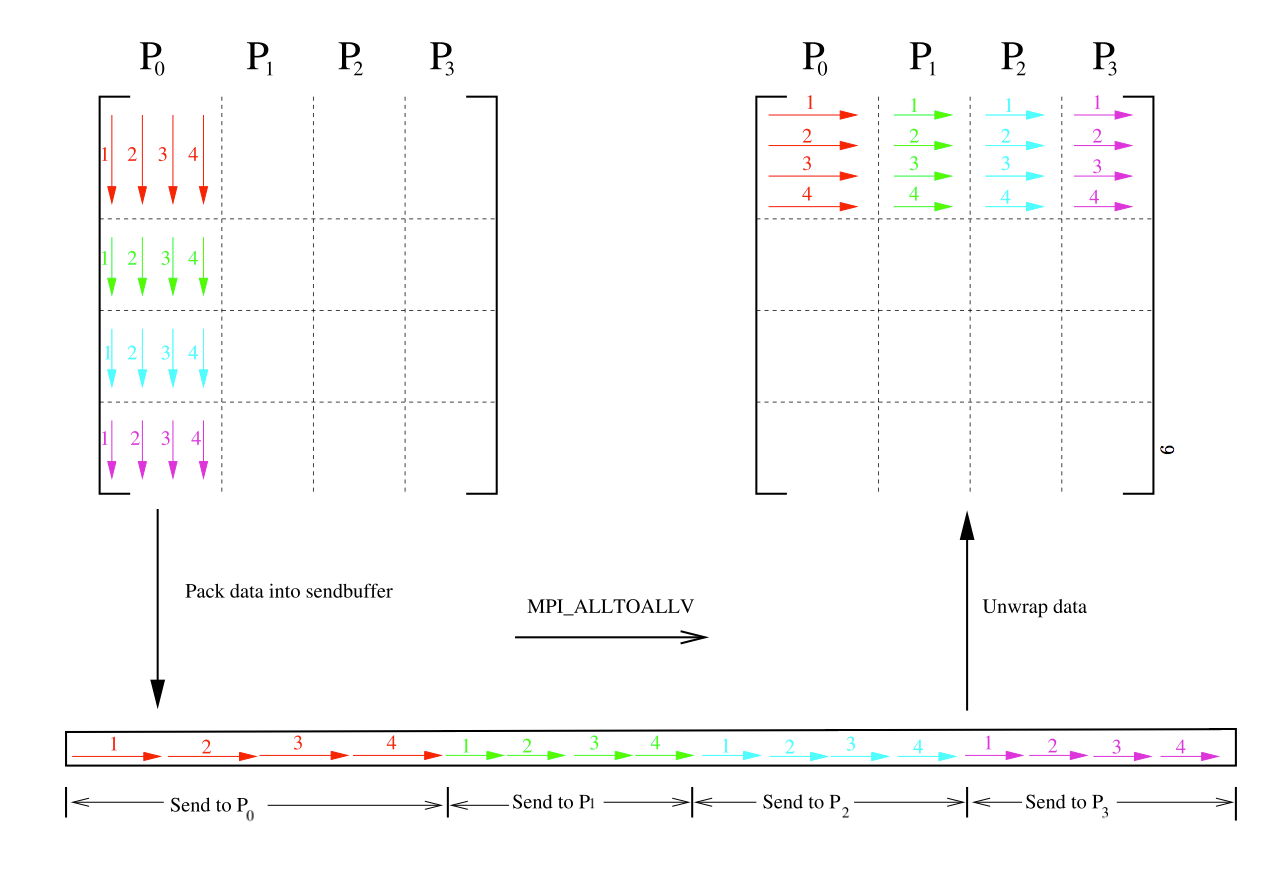
\includegraphics[scale=0.3]{transpose.png}
\caption{Figur hentet fra oppgaveteksten om transponeringen}
\end{figure}

Når beregningene er ferdige er resultatene spredd utover prosessene. Løsningen består


    % På maskiner med distrubuert minne kan vi dra nytte av MPI-biblioteket\cite{MPI} for å løse ligningssystemet. Ved å dele opp kolonnevis etter behov kan vi gjøre sinustransformasjonen parallelt. Utfordringen blir da å transponere matrisen på tvers av prosesser med MPI. Kolonnene hver enkelt prosess har tilgang til gjøres om til en vektor og sendes oppdelt med MPI\_Alltoallv til de respektive prosesser. Prosessen som mottar vektoren pakker denne ut til sin del av matrisa og kan gjøre videre beregninger.

    % Videre kan ytterligere forbedringer gjøres for å forbedre parallelliteten. Ved å bruke OpenMP\cite{MP} kan vi bruke flere tråder innen hver prosess slik at sinustransformasjonen gjennomføres ved en høyere grad av parallellitet. Her dukker det opp en utfordring med minnebruk da hver tråd krever en del av minne for å kunne utføre sinustransformasjonen.

    \subsection{Speedup og parallellitet}

    \section{Resultater}

    \section{Analyse}

    \section{Konklusjon}


% EXAMPLE OF CODE INCLUSION: \lstinputlisting[language=C, firstline=53, lastline=71, caption=MPI version]{../src/oving4-openmpi.c}

%----------------------------------------------------------------------------------------

\begin{thebibliography}{99}

\bibitem{ky}
Erwin Kreyzig,
\emph{Advanced Engineering Mathematics}.
9th Edition,
2006.

\bibitem{MPI}
OpenMPI, Open Source High Performance Computing, \it{http://www.open-mpi.org/}, 12.04.2013

\bibitem{MP}
OpenMP, \it{http://www.open-mpi.org/}, 12.04.2013
\end{thebibliography}

\end{document}